% Para documento texto corto
%\documentclass[paper=letter,oneside,fontsize=12pt]{article}
\documentclass[paper=letter,oneside,fontsize=11pt]{article}
%\documentclass[paper=letter,oneside,fontsize=11pt, parskip=full]{scrartcl}
%\documentclass[paper=letter,oneside,fontsize=12pt]{scrartcl}

% Permite visualizar el layout del documento
% \usepackage{showframe}


% Establecer dimensiones de los margenes
%\ usepackage[inner=1.5cm,outer=3cm,top=2cm,bottom=4cm,
%bindingoffset=5mm]{geometry}
\usepackage[left=3cm,right=3cm,top=3cm,bottom=3cm,
bindingoffset=0cm, footskip=0.5cm, headheight=2cm]{geometry}

% Elimina sangrias y aumenta espacio entre parrafos
\usepackage{parskip}

% Permite cambiar margenes derecho e izquierdo
% de secciones de texto con el entorno
% adjustwidth
\usepackage{changepage}

% Permite establecer el espaciado entre lineas
\usepackage{setspace}

% Establece separación entre parrafos
%\parskip=4pt

% Permite ingresar caracteres acentuados y especiales 
% sin necesidad de emplear comando
% utf8 codificacion de entrada Unicode (mas simbolos que ASCII)
\usepackage[utf8]{inputenc}

% T1 encoding for European, English, American text
\usepackage[T1]{fontenc}
% Fuente escalable
%\usepackage{lmodern}

% Reemplazo para fuente Arial
\usepackage{helvet}
\renewcommand{\familydefault}{\sfdefault}

% Formato direccione URL
% \usepackage{hyperref, xcolor}

% Carga babel, idioma ingles
\usepackage[english,spanish]{babel}

% Mejor jsutificacion, tipografia alta calidad.
\usepackage{microtype}
% Para unir columnas y filas en tablas
\usepackage{array}

% Agrega comandos extra al comando tabular
% \toprule, \midrule, \bottomrule
\usepackage{booktabs}
% Tablas con ancho establecido por usuario
\usepackage{tabularx}
% Para posicionamiento preciso de tablas dentro del texto
\usepackage{float}

% Encabezados personalizados
\usepackage{fancyhdr}
\usepackage{graphicx}

% Permite obtener el numero de la ultima pagina
\usepackage{lastpage}

% Paquetes para figuras
% Paquete caption para titulos figuras
% Paquete subcaption para subfiguras
\usepackage{caption}
\usepackage{subcaption}

% Espaciado inteligente
\usepackage{xspace} 

% Para formato de codigo fuente
\usepackage{xcolor}
\usepackage{listings}
\lstset{basicstyle=\ttfamily,
	showstringspaces=false,
	commentstyle=\color{red},
	keywordstyle=\color{blue}}

% Cabeceras
\pagestyle{fancy}
% Borra cabecera y pie actuales
\fancyhead{}
% Cintillo cabecera
%\chead{
%	
\includegraphics[width=150mm]{Imagenes/Cabecera.png}
%}
\fancyhead[L]{\includegraphics[width=0.3\textwidth]{Imagenes/cabecera.pdf}}
\fancyfoot[C]{ 
	\begin{tabularx}{\textwidth}{|m{3.0cm}|X|m{2.5cm}|m{1.0cm}|}
		\hline			
			\centering
			\includegraphics[height=0.8cm]{Imagenes/pie-izq.pdf} &			
			\centering
			Confidencial &
			\centering
			\includegraphics[height=0.8cm]{Imagenes/pie-der.pdf}  &			
			\thepage~/~\pageref{LastPage} \\
		\hline 
	\end{tabularx}	 
}

% Comando para formatear y justificar parrafos de código y 
% comandos de shell

\newcommand{\code}[1]{
	\begin{adjustwidth}{1.5cm}{0.0cm}
		\ttfamily
		#1
\end{adjustwidth}}	


% Numeracion de paginas
% numeros arabigos
\pagenumbering{arabic}

\begin{document}
	
	%\begin{titlepage}		
	
	\begin{center} 
		
		\vspace{10cm}
		
		\begin{Large} 
			\textsc{Dirección de Servicios de Certificación}
			\vspace{5pt}
			\begin{spacing}{0.9}
				\textsc{Laboratorio de Ensayos de Compatibilidad~Electromagnética~Radiada}
			\end{spacing}
		\end{Large}
		
		%\vspace{10cm}
		\vfill
		
		
		\begin{LARGE}	
			\begin{spacing}{0.9}		
				\textsc{Instalación del adaptador USB / GPIB Agilent~82357B en linux}
			\end{spacing}
		\end{LARGE}			
		\vspace{5pt}
		\begin{large}			
			\textsc{Construcción de la librería linux-gpib y carga de firmware}
		\end{large}	
	
		\vfill

		
		\begin{table}[!b]
			\begin{tabularx}{\linewidth}{|X|X|X|X|}	
				\hline				
				\multicolumn{2}{|l|}{\textbf{CÓDIGO}: FO-IT-002} & \multicolumn{2}{l|}{\textbf{N DOC:}} \\
				\hline
				Originado por:	& 	Elaborado por: & 
				Revisado por: 	& 	Aprobado por: \\
				\hline
				Br. Arias B., Jose A. & Br. Arias B., Jose A. & - & - \\
				\hline
				\textbf{Fecha: 20/06/2017 } & 
				\textbf{Fecha: 20/06/2016} & 
				\textbf{Fecha: } &
				\textbf{Fecha: } \\				
				%\hline
			\end{tabularx}	
		\end{table}	
		
		\vspace{10mm}
		
	\end{center}
	
	%\end{titlepage}
	
	\clearpage
	
	\tableofcontents
	
	\section{Objetivos}
		\begin{itemize}
			\item  Describir el proceso de instalación adaptador USB/GPIB Agilent 82357B en Ubuntu LTS 14.
			\item Instalar y construir, a partir del código fuente, la librería c de soporte (linux-gpib).
			\item Obtener los archivos de código fuente y contruir la utilidad de linux \texttt{fxload}, cargador de firmware para dispositivos USB.
			\item Obtener los archivos binarios y cargar el firmware para el dispositivo 82357B.
		\end{itemize}
		
	\section{Alcance}
	
		Describe el proceso de instalación adaptador USB/GPIB Agilent 82357B, la instalación y construcción de la librería c de soporte (linux-gpib) a partir del código fuente y la obtención y carga del firmware para el adaptador.	
		
	\section{Documentos de referencia}

	\subsection{Pagina raíz para la librería linux-gpib}	
	
	\texttt{http://linux-gpib.sourceforge.net/}
	
	\subsection{Enlace para código fuente linux-gpib}
	
	A la fecha de este documento, se encuentra el código fuente para la librería linux-gpib en la versión 4.0.4,	
	
	\texttt{https://sourceforge.net/projects/linux-gpib/files/}

	
	\subsection{Descripción del proceso para obtención y carga del firmware para el adaptador USB/GPIB 82357B}
	
	\texttt{https://gist.github.com/turingbirds/6eb05c9267a6437183a9567700e8581a}
	
	\texttt{http://git.net/ml/linux.hardware.gpib.general/2008-02/msg00001.html}
	
	\subsection{Instalación de los archivos de cabecera para el núcleo linux}

	Instalación de los  archivos de cabecera para el núcleo (kernel) apropiado al numero de versión de la distribución de linux que se utilice
	
	\texttt{https://www.cyberciti.biz/faq/howto-install-kernel-headers-package/}
	
	\texttt{http://git.net/ml/linux.hardware.gpib.general/2008-02/msg00001.html}
	
	\section{Términos y definiciones}
	
	\begin{tabular}{rl}
		Shell 	& 	Terminal de linux \\
		GPIB 	& 	General Purpouse Instrumentation Bus \\
		USB		&  	Universal Serial Bus \\
	\end{tabular}
	
	\section{Personal autorizado}	
		Personal técnico Cendit con interés en el uso del dispositivo
		
	\section{Personal requerido}	
		Todo aquel personal técnico Cendit con interés en el uso del dispositivo
		
	\section{Materiales}
		\label{Sec:SeccionMateriales}
		\begin{itemize}
			\item Adaptador USB / GPIB Agilent 82357B.
			\item Computador personal con puerto USB y acceso a internet.
		\end{itemize}	
			
	\section{Herramientas y equipos}
		
		Ver sección \ref{Sec:SeccionMateriales}.

	
	\section{Equipos de protección personal}
	
		No se requieren equipos protección personal.
		
	\section{Precauciones de seguridad}
	
		Para ejecutar esta actividad no se preveen precauciones de seguridad
		
	\section{Descripción de la actividad}
	
		\subsection{Generalidades}
	
		El adaptador USB / GPIB modelo 82357B, de Agilent Technologies como el mostrado en la figura \ref{Fig:AdaptadorGpibUsb} permite conectar un computador a un bus GPIB. Para poder utilizar este dispositivo se requiere que en el computador este instalado el software que le sirve de soporte, como lo son el modulo de kernel y las librerías de usuario.	
		
		\begin{figure}[!h]
			\begin{center}
				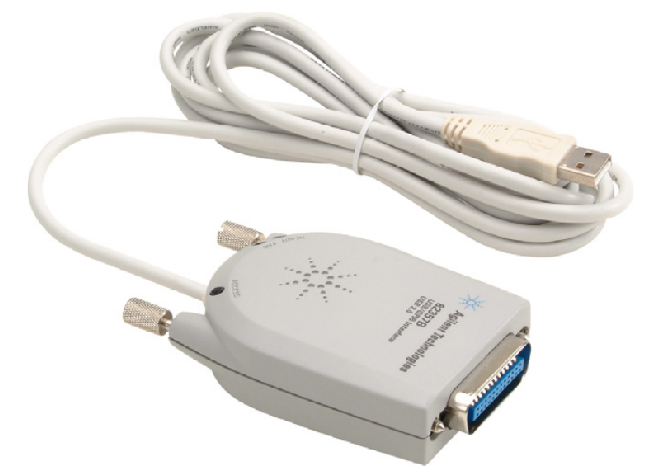
\includegraphics[width=8cm]{Imagenes/AdaptadorGpibUsb.pdf}
				\caption{Adaptador USB GPIB 82357B de Agilent Technologies}
				\label{Fig:AdaptadorGpibUsb}
			\end{center}
		\end{figure}	
		
		La empresa Keysight Technologies (antigua Agilent) proporciona un conjunto de herramientas de software, conocido bajo el nombre de \emph{IO Libraries Suite}, de libre descarga en el sitio web de esta empresa en la version 6.2017, a la fecha de redactar esta nota.
		
		IO Libraries Suite proporciona el software necesario para el intercambio de datos con instrumentos programables a través de buses RS232, GPIB, USB y redes LAN. El software se presenta en forma de utilidades ejecutables que permiten enviar comandos a los instrumentos y recibir sus respuesta, resolución de problemas así como también un librerías para desarrollo de aplicaciones.
		
		Las librerías \emph{VISA} (Virtual Instruments Software Architecture) proporcionan una capa de software uniforme desde el punto de vista del programador, para el acceso a los buses mencionados. La librería VISA es parte integral de IO Libraries Suite. Existen librerias VISA producidas por otras empresas del ramo de la instrumentación inteligente, una de las más reconocidas es la libreria VISA de National Instruments (NI-VISA) asi como también la librería VISA de Tektronix.
		
		El software proporcionado por Keysight Technologies es exclusivo para ambiente Windows. Las librerías VISA de National Instruments estan dirigidas Windows y a ciertas distribuciones de Linux, pero no para Ubuntu.
		
		Existe una alternativa, la librería \emph{linux-gpib} 
		
		Para utilizar el dispositivo adaptador USB / GPIB se requiere el siguiente soporte de software
		
		\begin{itemize}
			\item El soporte a nivel de librerías de usuario (user space) en el PC, en Ubuntu se recurre a \emph{linux-gpib}.
			\item El soporte de software a nivel de núcleo de sistema (kernel)en el PC, los moduleos de núcleo ().
			\item El soporte a nivel de firmware en el dispositivo Agilent 82357B, es necesario cargar una versión actualizada del firmware para este dispositivo.
		\end{itemize}
	
		\subsection{Instalación de linux-gpib y módulos de núcleo}
		
		La librería linux-gpib se construirá a partir de su código fuente, el cual puede descargarse de forma libre en el siguiente enlace
		
			
		\code{https://sourceforge.net/projects/linux-gpib/?source=dlp}

		
		Como requisito para construir esta librería, en el sistema deben estar instalados los archivos de cabecera del núcleo, apropiado para la versión de núcleo de linux que se este utilizando. El comando \texttt{uname} de shell de linux permite obtener la versión de núcleo que se este utilizando:
		
		\code{uname -r}
		
		Por medio del siguiente comando de shell se instalan los archivos de cabecera, acordes a la versión de linux:
		
		\code{sudo apt-get update \\		
		sudo apt-get install linux-headers-\$(uname -r)}
		
		Si se desea tener acceso a esta librería por medio de Python, se debe instalar el paquete \texttt{python-setuptools}: 
		
		\code{sudo apt-get install python-dev libboost-python-dev python-setuptools --yes}
		
		Ahora se procede a la descarga de los archivos fuente para la libreria \texttt{linux-gpib}, puede hacerse sin salir del shell por medio del comando \texttt{wget}. Se puede crear un directorio nuevo para almacenar los archivos descargados, ejecutando previamente \texttt{mkdir nombre\_directorio}.
		
		\code{wget --content-disposition --no-check-certificate \\
			\indent https://sourceforge.net/projects/linux-gpib/files/latest/download?source=dlp}
		
		El paso siguiente es descomprimir el archivo mediante el comando de shell \texttt{tar}, como se indica a continuación, en donde se debe introducir el nombre del archivo comprimido el cual indica la versión, en este caso se trata de la versión 3.2.20:
		
		\texttt{tar xvfz tar xvfz linux-gpib-3.2.20.tar.gz}
		
		Ahora se procede a construir la librería, por medio de la secuencia de comandos:
		
		\texttt{./configure}
		
		\texttt{make -j8} 
		
		\texttt{make install}
		
		Comprobar
		
		\texttt{whereis libgpib.so}
		
		Debe responder mostrando la ruta donde se encuentra la libreria, en Debian:
		
		\texttt{libgpib: /usr/local/lib/libgpib.so /usr/local/lib/libgpib.la}	
		
		\subsection{Instalación de módulos de núcleo}
		
		El módulo de núcleo llamado \texttt{agilent\_82357a.ko} también fue instalado durante el procedimiento de construcción del código fuente en el paso anterior. Se encuentra localizado en el PC donde se edita este documento en \texttt{/lib/modules/3.16.0-4-amd64/gpib/agilent\_82357a}, en esta ruta el subdirectorio con nombre \texttt{3.16.0-4-amd64} indica la versión de núcleo del PC (3.14) y su arquitectura (amd64). 
		
		Se procede a cargar el modulo de núcleo con el comando de shell \texttt{modprobe}, de la siguiente forma:
		
		\texttt{sudo modprobe agilent\_82357a}
		
		Si la carga ocurre de forma correcta, el comando no genera ninguna repuesta. Asi que se debe revisar si el módulo ha sido cargado de forma adecuada, por medio de los siguientes comandos de shell:
		
		\texttt{lsmod | grep agilent}
		
		Este comando emite una repuesta similar a la siguiente:

		\begin{flushleft}			
		%\begin{minipage}{\textwidth}
		%\begin{lstlisting}[language=bash]	
		\begin{ttfamily}	
			agilent\_82357a	22661  0 \\				
			gpib\_common	35582  1 agilent\_82357a  \\				
			usbcore	195468  4 uhci\_hcd,agilent\_82357a,ehci\_hcd,ehci\_pci \\
		\end{ttfamily}
		%\end{lstlisting}
		%\end{minipage}		
		\end{flushleft}
		
		La primera línea de la salida del comando \texttt{lsmod} indica que el módulo \texttt{agilent\_82357a} se ha cargado correctamente. 	
		
		El comando de shell \texttt{modinfo} 
		
		https://twiki.cern.ch/twiki/bin/view/Main/GpibLinux
		
		\subsection{Instalación de archivos binarios de firmware para el 82357B}
		
		https://gist.github.com/turingbirds/6eb05c9267a6437183a9567700e8581a
		
		Para que el dispositvo 82357B funcione correctamente debe actualizarse su firmware. Los archivo binarios para el firmware se encuentran 
		
		\texttt{http://linux-gpib.sourceforge.net/firmware/gpib\_firmware-2008-08-10.tar.gz}
		
		Se descargan los binarios comprimidos y se descomprimen con los acostumbrados comandos \texttt{wget} y \texttt{tar}:
		
		\texttt{wget 		https://gist.github.com/turingbirds/6eb05c9267a6437183a9567700e8581a}
		
		\texttt{tar xvfz gpib\_firmware-2008-08-10.tar.gz}
		
		Ahora se procede a descargar el codigo fuente de la utilidad \texttt{fxload}. El procedimiento es similar a los mostrados anteriormente, se descarga el archivo comprimido, se descomprime para luego construir el código fuente de la forma acostumbrada en entornos linux. El enlace para el código fuente de \texttt{fxload} se encuentra en el siguiente enlace:
		
		\texttt{https://downloads.sourceforge.net/project/linux-hotplug/fxload/2008\_10\_13/fxload-2008\_10\_13.tar.gz}
		
		Se descarga de este enlace el código fuente con el comando de shell \texttt{wget}:
		
		\texttt{wget --content-disposition --no-check-certificate https://downloads.sourceforge.net/project/linux-hotplug/fxload/2008\_10\_13/fxload-2008\_10\_13.tar.gz}
		
		Se descomprime el archivo:
		
		\texttt{tar xvfz fxload-2008\_10\_13.tar.gz}
		
		Ahora se ingresa al subdirectorio \texttt{fxload-2008\_10\_13} en donde se encuentra el códifo fuente:
		
		\texttt{cd fxload-2008\_10\_13}
		
		Se construye el mismo por medio de los comandos:
		
		\texttt{make}
		
		\texttt{sudo make install}
		
		Se deben editar dos lineas en el archivo \texttt{/etc/gpib.conf} para indicar el tipo de adaptador y asignarle un nombre que permita identificar el adaptador por una cadena en vez de una dirección GPIB numérica. El usuario puede elegir cualquier nombre que desee.
		
		\texttt{board\_type = "agilent\_82357a"}
		
		\texttt{name = "AGILENT82357B"}
		
		\texttt{pad = 22}
		
		Se cargan los módulos de núcleo:
		
		\texttt{sudo modprobe gpib\_common}
		
		\texttt{sudo modprobe agilent\_82357a}
		
		Ahora se procede a insertar el dispositivo 82357B en el puerto USB del PC, en éste solo debe encontrarse iluminado en rojo el LED FAIL. 
		
		Por medio del comando \texttt{lsusb} se encuentran el \emph{identificador (ID) de bus} y el \emph{ID de dispositivo}, dentro de la ventana de shell se ejecuta
		
		\texttt{lsusb}
		
		El comando arroja varias entradas como respuesta, en una de ellas se debe encontrar la entrada para el adaptador de Agilent Technologies, similar a la que se muestra a continuación
	
		\texttt{Bus 002 Device 005: ID 0957:0518 Agilent Technologies, Inc.}
		
		De esta linea se observa que el sistema operativo se infiere que el ID de bus es el valor 002 y el ID de dispositivo es el valor 005. Se requieren estos datos en los argumentos del comando \texttt{fxload}.
		
		El archivo con extensión \emph{.hex} que contiene el firmware para el dispositivo se llama \texttt{measat\_releaseX1.8.hex}. Por medio del siguiente comando ejecutado dentro del shell se carga el firmware
		
		\texttt{sudo fxload -D /dev/bus/usb/002/005  -t fx2 -I gpib\_firmware-2008-08-10/agilent\_82357a/measat\_releaseX1.8.hex}
		
		En el dispositivo 82357B el LED FAIL debe estar iluminado en rojo aún. Se debe proceder a una nueva carga del firmware. Por medio del comando \texttt{lsusb} se obtienen por segunda vez el id de bus y el id de dispositivo
		
		\texttt{lsusb}
		
		El comando genera la respuesta
		
		\texttt{Bus 002 Device 006: ID 0957:0518 Agilent Technologies, Inc.}
		
		El id de bus debe ser el mismo (Bus 002), el valor que debería haber cambiado es el id de dispositivo (Device 006). Se procede nuevamente a ejecutar \texttt{fxload}, introduciendo en el argumento de este comando los valores de id de bus y id de dispositivo.
		
		\texttt{sudo fxload -D /dev/bus/usb/002/006  -t fx2 -I gpib\_firmware-2008-08-10/agilent\_82357a/measat\_releaseX1.8.hex}
		
		
		Como resultado de la ejecución del comando, en el dispositivo 82357B todos los LEDs deben encontrarse encendidos.		
		
		Se deben cambiar los permisos sobre el archivo que representa el acceso al disposotivo USB / GPIP ubicado en la ruta \texttt{/dev/gpib0}, por medio del comando
		
		\texttt{sudo chmod 666 /dev/gpib0}
		
		Resta inicializar el dispositivo 82357B por medio del comando \texttt{gpib\_config}. Este comando tiene ciertos problemas en ubicar la librería \texttt{libgpib.so}, así que se debe crear un \emph{enlace simbólico} de la siguiente forma
		
		\texttt{sudo ln -s /usr/local/lib/libgpib.so.0 /lib/libgpib.so.0}
		
		Para ahora ejecutar el comando
			
		\begin{ttfamily}
			\texttt{gpib\_config}
		\end{ttfamily}

	
		Como resultado de procedimiento en el dispositivo 82357B se debe encontrar el LED READY iluminado en verde.
	
	\section{Anexos}	
		
\end{document}